\documentclass[border=10pt]{standalone}
\usepackage{tikz}

%%\usepackage{helvet}

\begin{document}
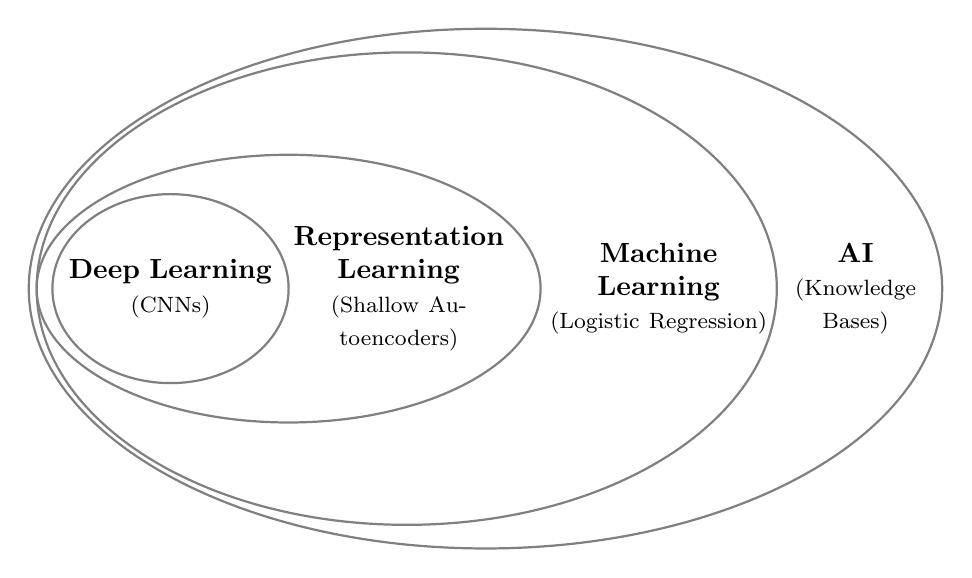
\begin{tikzpicture}[thick]

\begin{scope}[gray]
  \draw[thick] (5,1) circle [x radius=5.8cm, y radius=3.3cm];
  \draw[thick] (4,1) circle [x radius=4.7cm, y radius=3.cm];
  \draw[thick] (2.5,1) circle [x radius=3.2cm, y radius=1.7cm];
  \draw[thick] (1,1) circle [x radius=1.5cm, y radius=1.2cm];
\end{scope}

\begin{scope} %[white]
  \node[align=center,text width=3cm,in front of path] at (1,1)    {\textbf{Deep Learning}\\\footnotesize{(CNNs)}};
  \node[align=center,text width=3cm,in front of path] at (3.9,1)    {\textbf{Representation Learning}\\\footnotesize{(Shallow Autoencoders)}};
  \node[align=center,text width=3cm,in front of path] at (7.2,1)    {\textbf{Machine Learning}\\\footnotesize{(Logistic Regression)}};
  \node[align=center,text width=2cm,in front of path] at (9.7,1)    {\textbf{AI}\\\footnotesize{(Knowledge Bases)}};
\end{scope}
  
\end{tikzpicture}
\end{document}
